\section{Listener\-Func Class Reference}
\label{classListenerFunc}\index{ListenerFunc@{ListenerFunc}}
Inheritance diagram for Listener\-Func::\begin{figure}[H]
\begin{center}
\leavevmode
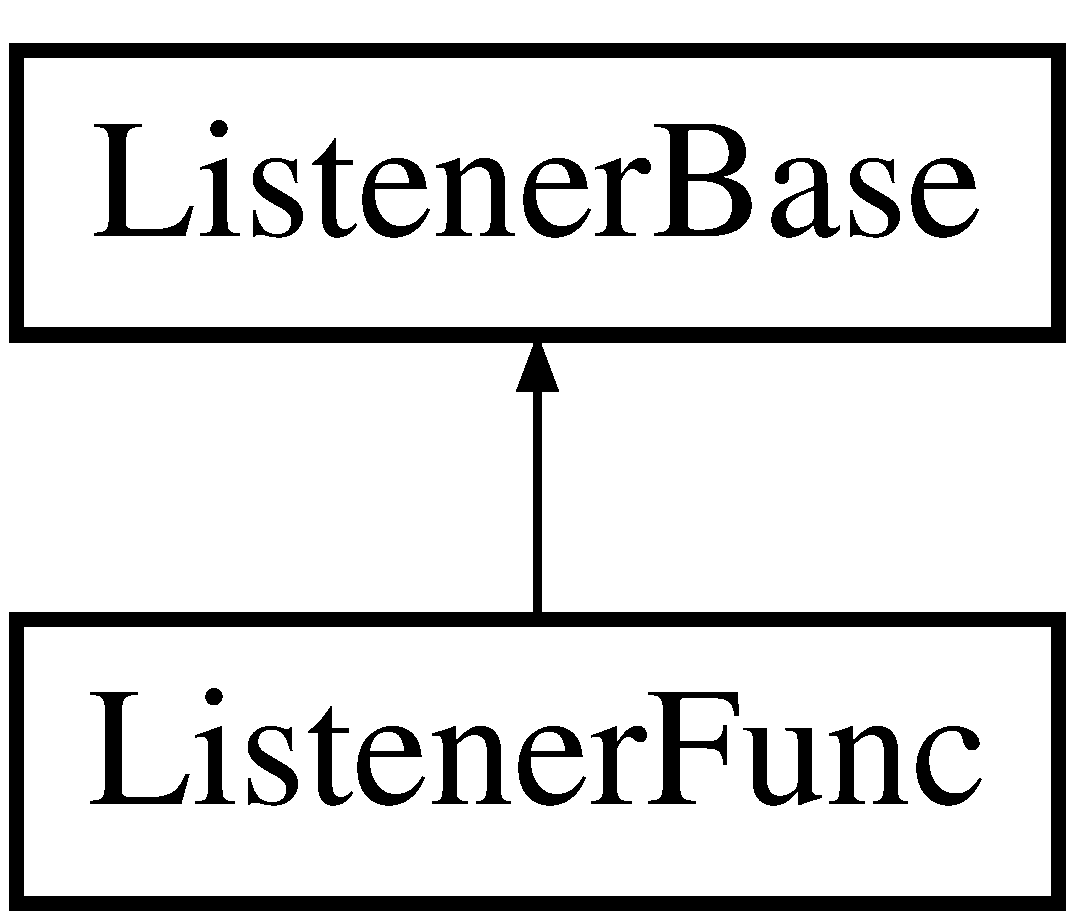
\includegraphics[height=2cm]{classListenerFunc}
\end{center}
\end{figure}
\subsection*{Public Member Functions}
\begin{CompactItemize}
\item 
{\bf \_\-\_\-del\_\-\_\-} ()
\item 
{\bf invoke} ()
\end{CompactItemize}


\subsection{Member Function Documentation}
\index{ListenerFunc@{Listener\-Func}!__del__@{\_\-\_\-del\_\-\_\-}}
\index{__del__@{\_\-\_\-del\_\-\_\-}!ListenerFunc@{Listener\-Func}}
\subsubsection{\setlength{\rightskip}{0pt plus 5cm}Listener\-Func::\_\-\_\-del\_\-\_\- ()}\label{classListenerFunc_ListenerFunca0}


\index{ListenerFunc@{Listener\-Func}!invoke@{invoke}}
\index{invoke@{invoke}!ListenerFunc@{Listener\-Func}}
\subsubsection{\setlength{\rightskip}{0pt plus 5cm}Listener\-Func::invoke ()}\label{classListenerFunc_ListenerFunca1}




Reimplemented from {\bf Listener\-Base} {\rm (p.\,\pageref{classListenerBase_ListenerBasea0})}.

The documentation for this class was generated from the following file:\begin{CompactItemize}
\item 
{\bf Listener.py}\end{CompactItemize}
